\documentclass{article}
\usepackage{graphicx} % Required for inserting images
\usepackage{parskip} 
\usepackage{enumitem}
\usepackage{calc}     % needed for \widthof
\usepackage{subcaption}
\usepackage{float}
\usepackage{tabularx}
\usepackage{placeins}
\usepackage{listings}
\usepackage{xcolor}
\usepackage{ragged2e}
\usepackage{url}

\graphicspath{{Architecture}{Components}{Deployment}{Sequence_Diagrams}}


\title{
\vspace{-1cm}
\includegraphics[width=0.25\textwidth]{Logo_Politecnico_Milano.png}\\[1cm]
\textbf{Design Document}\\
\textbf{DD}\\
\vspace{0.4cm}
\large Best Bike Paths
}

\author{Cristian Summa \and Mathias Rodigari}

\date{
Software Engineering II\\
\vspace{0.3cm}
Academic Year 2025--2026
}

\begin{document}

\maketitle

\newpage

\tableofcontents

\newpage

\section{Introduction}
    \subsection{Purpose}
        In contemporary urban environments, cycling has emerged as a widespread and sustainable mode of transportation, embraced by commuters, enthusiasts, and casual riders alike. As cities increasingly promote eco-friendly mobility, cyclists face growing challenges related to route safety, path quality, and access to reliable information. Despite the abundance of bike paths, riders often lack a clear and comprehensive understanding of which routes best suit their needs, preferences, and riding conditions.

        At the same time, the rise of personal activity tracking has highlighted the importance of understanding individual performance and travel habits. However, existing solutions frequently separate personal trip monitoring from shared, community-driven knowledge about cycling infrastructure, limiting their overall usefulness.
        
        Best Bike Paths (BBP) is designed as an integrated platform that bridges this gap by combining personal ride tracking with collaborative mapping of bike path conditions. The system enables cyclists to record and analyse their trips while actively contributing to a shared repository of information regarding path quality, obstacles, and overall cycling experience. By leveraging both individual data and collective insights, BBP supports informed route selection and fosters a more transparent and reliable cycling environment.
    
        Through this unified approach, BBP aims to enhance the overall cycling experience, empowering users to navigate urban spaces with greater confidence, safety, and awareness, while promoting a community-oriented model of sustainable mobility.

    \subsection{Scope}
        The scope of Best Bike Paths (BBP) is to provide a unified and reliable platform that supports cyclists in both documenting their personal riding activities and accessing shared knowledge about bike path conditions. The system acts as an intermediary between individual users and the collective information generated by the cycling community, enabling the aggregation, validation, and dissemination of path-related data.

        BBP is accessed by two categories of external users: registered users and unregistered users. Registered users interact with the system through personal accounts, which allow them to record cycling trips, store historical activity data, and actively contribute information about bike paths. Unregistered users, instead, can freely explore the system to discover available routes between locations, benefiting from the information collected by the community without contributing data themselves.

        The platform supports both manual and automated data acquisition. Registered users may manually insert details regarding the characteristics, conditions, and status of bike paths, or initiate automated tracking sessions during their rides. In the latter case, the system collects data through the device’s sensors to reconstruct the travelled route and detect potential obstacles or hazards. To ensure the reliability of shared information, automatically acquired data must be reviewed and confirmed by users before being published and made available to the wider community.

        In addition to trip recording and data contribution, BBP provides route discovery functionalities for all users. Given an origin and a destination, the system analyses the available path information and identifies viable bike routes, prioritizing those that are safer, better maintained, or more suitable based on community feedback and reported conditions.

        By integrating personal activity tracking, collaborative data contribution, and intelligent route discovery, BBP establishes a structured environment in which cyclists can both contribute to and benefit from continuously updated knowledge, enhancing navigation, safety awareness, and the overall cycling experience.

        \subsection{Definitions, Acronyms, Abbreviations}
            \subsubsection{Definitions}
                    \begin{description}[style=unboxed, font=\bfseries, labelwidth=\linewidth, labelsep=0pt, leftmargin=0pt, itemsep=0.8em, align=left]
                    \item[Path\hfill]
                    A segment of road or bike infrastructure considered safe for cycling. It may consist of a dedicated bike lane, a road where motor vehicles are restricted, or a street where traffic conditions (e.g., low speed limits) allow safe coexistence with cars.
    
                    \item[Trip\hfill] 
                    A cycling activity performed by a user, consisting of movement across one or more paths or streets. A trip has a clearly defined start and end time and may include additional recorded information such as distance, average speed, weather, etc.
                    
                    \item[User\hfill] 
                    Any individual interacting with the system. Depending on the type of interaction, the system distinguishes between registered and unregistered users.
                
                    \item[Registered User\hfill] 
                    A user who has created an account. Registered users can record trips, insert path-related information, initiate tracking sessions, and access personal data history.
                
                    \item[Unregistered User\hfill] 
                    A user who interacts without an account. They can browse paths, search routes, and record trips locally, but cannot save trips or contribute path information.
                    
                    \item[Path Status\hfill] 
                    A qualitative evaluation of a path’s condition using categories (optimal, medium, sufficient, requires maintenance). Reflects surface quality, safety, and usability.
                
                    \item[Obstacle\hfill] 
                    Any element along a path that may impede or endanger a cyclist, like potholes, bumps, debris, or irregularities. Can be reported manually or inferred via sensors.
                
                    \item[Tracking Session\hfill] 
                    A user-initiated recording mode collecting sensor data (GPS, accelerometer, gyroscope) to reconstruct the route and detect obstacles.
                
                    \item[Sensor Data\hfill] 
                    Information collected during a tracking session, including GPS location, speed, acceleration, and orientation, used to reconstruct paths and detect obstacles.
                \end{description}

            \subsubsection{Acronyms}
                \begin{description}[
                leftmargin=2em, 
                labelindent=2em, 
                labelwidth=\widthof{\bfseries SSO}
                ]
                  \item[\textbf{BBP}] Best Bike Paths
                  \item[\textbf{GPS}] Global Positioning System
                  \item[\textbf{API}] Application Programming Interface
                  \item[\textbf{DB}] Database
                  \item[\textbf{UI}] User Interface
                  \item[\textbf{UX}] User Experience
                  \item[\textbf{OS}] Operating System
                  \item[\textbf{SSO}] Single Sign On
                  \item[\textbf{DBMS}] DataBase Management System
                \end{description}

        \subsection{Revision History}
            \begin{description}
                \item[Version 1 - 07/01/2026]\mbox{}\\
                Initial release of the document.
            \end{description}

        \subsection{Reference Documents}
            This document and the information contained herein refer to the following sources:
            \begin{itemize}
                \item Requirement Engineering and Design Project Specification, Software Engineering II course, Academic Year 2025/26.
                \item Course slides and materials available on the WeBeep page of the Software Engineering II course.
            \end{itemize}
            

        \subsection{Document Structure}
            This document is organized as follows:
            \begin{enumerate}
                \item \textbf{Introduction:} This section provides a brief description of the project. In particular, it focuses on the motivations behind the development of Best Bike Paths (BBP), as well as on the goals and objectives that the system aims to achieve, in accordance with what has been defined in the Requirements Analysis and Specification Document (RASD).
                \item \textbf{Architectural Design:} This section describes the architectural design of the system at different levels of granularity. It presents the main architectural choices adopted for BBP, the decomposition of the system into components, and the interactions among them, providing a technical overview of how the system is structured.
                \item \textbf{User Interface Design:} This section illustrates the design of the user interface of the BBP platform. It includes high-fidelity mockups and descriptions of the main screens, showing how users interact with the system and access its functionalities.
                \item \textbf{Requirements Traceability:} This section explains how the goals defined in the RASD are satisfied by the system design. It highlights the relationships between goals, requirements, and architectural components, ensuring traceability between analysis and design decisions.
                \item \textbf{Implementation, Integration, and Test Plan:} This section provides an overview of the implementation strategy, integration process, and testing activities. It describes how the different components of BBP are expected to be developed, integrated, and validated to ensure correct system behavior.
                \item \textbf{Effort Spent:} This section reports the effort spent by each member of the group in the preparation of this document.
                \item \textbf{References:} This section lists all documents, tools, and resources that were consulted or used during the creation of this document
            \end{enumerate}

    \newpage

    \section{Architectural Design}

        \subsection{Overview}
            This section consists of a high-level description of the architecture of the system, of the single components and the interaction between the architectural layers. It also includes the modeling choices that have been taken to fulfill the functional and nonfunctional requirements defined in the RASD document.

            \subsubsection{System View}
                The architectural design chosen for the BBP platform is a \textbf{4-tier architecture}, which allows for a clear separation of concerns, scalability, and high availability. The four tiers consist of a presentation tier, two application tiers, and a data tier.

                The \textbf{presentation tier} resides entirely on the client side and is implemented through native mobile applications. It is responsible for handling user interaction and presenting information to the user.

                The \textbf{application layer}, located on the server side, is divided into two distinct tiers. The first tier represents the \textbf{front-facing application layer}, which includes the API Gateway and acts as the single entry point for client requests. The second tier hosts the \textbf{backend application services}, which implement the system’s core business logic following a microservices architectural style.

                The \textbf{data tier} is responsible for persistent data storage and consists of distributed databases and the DBMS required for their operation.

                Information flow within the system originates at the presentation tier, where users interact with the application through their mobile devices. Requests are sent to the API Gateway, which processes and routes them to the appropriate backend microservices. These services may retrieve or update data within the data tier before returning the processed results back through the API Gateway to the client application.

                The separation of the application layer into two tiers enables a more distributed and scalable architecture. In particular, the API Gateway tier can act as an \textbf{edge layer}, allowing requests to be handled closer to users geographically and routed to the most suitable backend service instance based on latency and load conditions.

                As the primary architectural style for the backend application tier, the system adopts a \textbf{microservices-based architecture}, which is well suited for systems that require rapid scaling and independent evolution of components. Both the application layers and the data layer are designed to be replicated across multiple machines to ensure availability, fault tolerance, and resilience.

                \begin{figure}[H]
                    \centering
                    \includegraphics[width=\textwidth]{Architecture/System_View.drawio.png}
                    \caption{System View diagram showing the 4 tier architecture}
                    \label{fig:system_view_diagram}
                \end{figure}

            \subsubsection{Detailed View}
                \textbf{Presentation Tier}

                The presentation tier consists of the \textbf{mobile client applications}, through which users interact with the system. These applications are responsible for rendering the user interface, collecting user input, accessing sensor data, and issuing HTTP requests to the server-side components of the platform.

                The presentation tier contains no business logic and communicates exclusively with the system through the API Gateway, ensuring a clear separation between client-side presentation concerns and server-side processing.

                \hfill
                
                \textbf{Application Tier – Front End (API Gateway / Edge Layer)}

                The front-end application tier represents the system’s point of contact with external clients and networks. Its main component is the \textbf{API Gateway}, which serves as the single public entry point for all client requests.

                The API Gateway is responsible for several cross-cutting concerns, including request routing, authentication and authorization, rate limiting, caching, and request aggregation. It ensures that incoming requests originate from authenticated and authorized users before forwarding them to the appropriate backend services.

                Additionally, this tier may act as a proxy for communication with external services required by the system, such as identity providers, mapping services, or notification systems. By centralizing these interactions, the platform reduces coupling between backend services and third-party APIs.

                This tier also contributes to system security by providing an additional protective layer that mitigates threats such as denial-of-service attacks or malformed requests before they reach the core application services. Multiple instances of the API Gateway can be deployed in different geographical regions, allowing requests to be routed to the most appropriate backend services in terms of latency and workload.

                \hfill

                \textbf{Application Tier - Back End}

                The back-end application tier hosts the core services of the system and is responsible for implementing the platform’s business logic. This tier is structured according to a \textbf{microservices architecture}, where each service represents a distinct functional area of the system.

                Each microservice is designed to be independently deployable, scalable, and replaceable, and exposes a well-defined REST API. Communication between services is performed through RESTful calls, enabling loose coupling and facilitating independent development and deployment.

                To ensure availability and fault tolerance, microservices are replicated and distributed across multiple machines. This allows the system to continue functioning even in the presence of partial failures and to dynamically scale based on workload.

                \hfill

                \textbf{Data Tier}

                The data tier is responsible for managing persistent data and providing efficient access to it for the application services. It consists of a set of \textbf{distributed and replicated databases}, each managed by an appropriate DBMS.

                In line with the microservices architecture, each backend service relies on a \textbf{service-specific database}, which stores data tailored to its functional requirements. This approach extends the decoupling of services to the data layer, improving performance and reducing inter-service dependencies.

                Due to the geographically distributed nature of the platform and the location-dependent characteristics of much of the stored data, databases are primarily responsible for data related to specific geographical areas. Nevertheless, synchronization mechanisms are provided to ensure that data can be accessed consistently across different regions when required.

                Both replication and redundancy are employed within the data tier to guarantee data availability, fault tolerance, and acceptable performance under varying load conditions.

                \begin{figure}[H]
                    \centering
                    \includegraphics[width=\textwidth]{Architecture/Detailed_View.pdf}
                    \caption{Detailed View diagram showing the 4 tier architecture and its components}
                    \label{fig:detailed_view_diagram}
                \end{figure}

        \subsection{Component View}
            The system is composed of multiple components distributed across the frontend and backend layers, each responsible for delivering a specific service. In addition, the system interacts with several external components, some accessed directly by the backend services and others by the client device itself.

            \subsubsection{Back-End Components}
                \begin{itemize}
                    \item \textbf{User Management Service}\\
                    This service manages user accounts and profiles, including access to user-related data. It is responsible for handling profile information as well as user-generated content within BBP, such as trips, path drafts, and favorite or recently used locations.
                    
                    \item \textbf{Authentication Service}\\
                    This service handles user authentication and authorization processes. It supports both internal authentication mechanisms and external authentication through third-party Single Sign-On (SSO) providers.
                    
                    \item \textbf{DBMS}\\
                    This component is responsible for managing persistent data storage. It provides controlled access to the databases and executes data retrieval and update operations on behalf of the backend services.
                    
                    \item \textbf{Push Notification Service}\\
                    This service manages push notification channels to which client applications can subscribe. It enables asynchronous, server-to-client communication by delivering notifications requested by other backend services.
                    
                    \item \textbf{Search Path Service}\\
                    This service is responsible for executing path-finding algorithms. Given a pair of input coordinates, it computes and returns the optimal path according to the system’s routing logic, without maintaining any additional application state.
                    
                    \item \textbf{Search Destination Service}\\
                    This service interacts with external map data providers to access databases of known locations. It supports the fuzzy search functionality used by the client application and provides location data for populating interactive map markers.
                    
                    \item \textbf{Search Street Service}\\
                    This service accesses external map data providers to retrieve street information based on textual input. It supports the manual path creation workflow by enabling users to search for streets by name.
                    
                    \item \textbf{Navigation Service}\\
                    This service manages turn-by-turn navigation functionality. It processes real-time location updates received from the client and generates navigation instructions that are sent back to the client during an active navigation session.
                    
                    \item \textbf{Record Trip Service}\\
                    This service is responsible for receiving and storing trip data once a trip has ended. It persists this data in the database and may also update aggregated or derived information related to existing paths when required.
                    
                    \item \textbf{Add Path Service}\\
                    This service manages the complete path creation workflow. In automatic mode, it configures the necessary parameters and initiates a navigation session. In manual mode, it validates user inputs and coordinates with supporting services, such as the Search Street Service. Upon completion, it stores the path as a draft and may forward it to the Path Review Management Service for further processing.
                    
                    \item \textbf{Path Review Management Service}\\
                    This service manages the path review lifecycle. It maintains a review queue, tracks the review status of each submitted path, and persists approved paths to the database.
                    
                \end{itemize}

            \subsubsection{Front-End Components}
                \begin{itemize}
                    \item \textbf{Mobile Application}\\
                    The mobile application represents the primary interface through which users interact with the BBP system. It is responsible for presenting data received from the server, initiating requests to the API Gateway, and interacting with external services provided by the mobile operating systems, including the map rendering provider and the health data provider.
                \end{itemize}

            \subsubsection{External Services}
                \begin{itemize}
                    \item \textbf{Identity Provider}\\
                    The Identity Provider offers authentication services through third-party Single Sign-On (SSO) mechanisms. The system integrates with external identity providers to allow users to authenticate using existing accounts, specifically Google and Apple, reducing the need for platform-specific credential management.

                    \item \textbf{Map Provider}\\
                    The Map Provider supplies geographical and map-related data required by the backend services. This includes information about locations, streets, and routing data, which are accessed by services such as path search and destination search.

                    \item \textbf{Map Rendering Provider}\\
                    The Map Rendering Provider is responsible for rendering maps within the client application. This functionality is provided directly by the mobile operating system and differs by platform: \textbf{Google Maps} is used on Android devices, while \textbf{MapKit} is used on iOS devices.

                    \item \textbf{Weather Provider}\\
                    The Weather Provider supplies meteorological data used by the system to enhance the user experience. Weather information may be integrated into route planning, navigation, or trip analysis features.

                    \item \textbf{Health Data Provider}\\
                    The Health Data Provider allows the mobile application to access health and activity data stored on the user’s device, subject to user consent. The system integrates with \textbf{Google Fit} on Android and \textbf{HealthKit} on iOS to retrieve relevant fitness and activity metrics.
                    
                    On Android devices, data access is performed through the \textbf{Health Connect platform}, which provides a unified API for third-party applications and ensures interoperability with other health and fitness services, such as \textbf{Samsung Health} and similar vendor-specific applications.

                    \item \textbf{Push Notification Provider}\\
                    The Push Notification Provider delivers push notifications from the backend to client devices. It enables asynchronous communication by allowing backend services to send notifications to users through platform-specific notification infrastructures.
                \end{itemize}

                \begin{figure}[H]
                    \centering
                    \includegraphics[width=\textwidth]{Components/Components_Diagram.pdf}
                    \caption{Diagram of the main Components}
                    \label{fig:components_diagram}
                \end{figure}

        \subsection{Deployment View}
            This chapter describes the deployment view of the BBP system. It outlines the system’s execution environment and details the geographical distribution of the hardware components that host the software components composing the application.

            \begin{figure}[H]
                \centering
                \includegraphics[width=\textwidth]{Deployment/Deployment_Diagram.pdf}
                \caption{Diagram of the deployment view}
                \label{fig:deployment_diagram}
            \end{figure}

            \textbf{Smartphone}\\
            A smartphone requires the official BBP client application, which is distributed through the \textbf{Google Play Store} or the \textbf{Apple App Store}, depending on the operating system.
            The application communicates with the BBP system over \textbf{HTTPS}, ensuring secure and encrypted data transmission.

            All client requests are first filtered through a \textbf{firewall} to protect the system from unauthorized or malicious traffic, and are then forwarded to a \textbf{load balancer}, which distributes incoming requests across multiple instances of the API Gateway to ensure scalability and availability.

            \hfill
            
            \textbf{Firewall}\\
            The firewall inspects incoming network traffic and blocks potentially harmful packets before they reach the system. Placed ahead of the load balancers, it ensures that only safe traffic enters the network, establishing a secure perimeter around the system.

            \hfill

            \textbf{Load Balancer}\\
            The load balancer distributes incoming requests across multiple edge servers (API Gateways) to optimize system performance, scalability, and reliability. It ensures traffic is evenly balanced, preventing any single server from becoming a bottleneck, and enhances the overall resilience of the system.

            \hfill

            \textbf{Edge Server}\\
            The Edge servers are dedicated to the API Gateway component and can be deployed on separate machines from the Application Servers, with the option to scale horizontally. They handle requests from BBP clients and forward them to the Application Servers via HTTP REST calls. Designed for wider distribution, these servers can cache geographically relevant information, such as streets, destinations, and points of interest, reducing the load on the Application Servers for frequently requested data.

            These servers inherit the same deployment structure as the Application Servers.

            \hfill

            \textbf{Application Server}\\
            This term refers to the servers running one or more of BBP’s main components. Each server hosts a Kubernetes instance, where each Pod runs a single microservice. This architecture allows individual services to scale independently based on workload, improving efficiency and performance. The servers also provide isolation between services, helping to contain faults and maintain system stability. Additionally, they support monitoring and logging for each microservice, enabling better observability and maintenance. Network access is managed to ensure secure communication between services and with external clients, while resource allocation is optimized to maximize utilization without impacting system reliability.

            \hfill

            \textbf{Database Server}\\
            Each Application Server connects to its dedicated Database Server, with specialized databases tailored to the microservices it hosts. 

            Given the system’s reliance on geographical information, each database primarily manages data relevant to its specific area of operation. However, background synchronization and defined data pathways ensure that all databases maintain global access to the full dataset. 
            
            The databases are designed for high availability and resilience, supporting replication and fault tolerance so that application servers always have access to up-to-date information, minimizing errors caused by data inconsistencies.

        \newpage
        \subsection{Runtime View}
            In this section, we describe the interaction between system components through sequence diagrams, one for each use case, in order to illustrate the main logical flow that leads to the execution of the requested functionality.

            For the sake of clarity and readability, several aspects that are essential in a production system are intentionally omitted from the diagrams. In particular, we do not explicitly represent the verification of user authorization and authentication for each request, even when required by the operation. All interactions are therefore assumed to be performed by an already authenticated and authorized user.

            Furthermore, we do not model error-handling scenarios, including invalid input parameters, unavailable external services (e.g., Identity Providers, Map or Weather services), network failures, or internal component errors. All interactions shown in the diagrams represent successful execution paths.

            Although some components, like the API Gateway and some microservices, may employ caching mechanisms to reduce latency and database load, this behavior is not represented. Instead, the diagrams depict the general case in which each request that requires persistent data involves access to the database, in order to clearly show data dependencies between components.

            Finally, when external services are involved (such as Identity Providers, map services, weather services, or push notification providers), they are modeled as abstract external components. The diagrams represent logical interactions with these services without committing to provider-specific APIs or protocols, which may differ across implementations.

            These simplifications allow the sequence diagrams to focus on the core functional behavior of each use case and on the responsibilities and interactions of the main system components, rather than on infrastructural and operational concerns.

            \begin{figure}[H]
                \textbf{[UC1] User Registration}\par\vspace{1em}
                \centering
                \includegraphics[width=\textwidth]{Sequence_Diagrams/UC1_User_Registration.png}
                \justifying
                This sequence diagram illustrates the flow of messages involved in the Sign In use case, covering both the internal authentication process based on email and password and the external authentication process performed through a selected Single Sign-On (SSO) provider. Upon successful completion of either flow, a corresponding User instance is created and stored in the database if it does not already exist.
            \end{figure}

            \begin{figure}[H]
                \textbf{[UC2] User Login}\par\vspace{1em}
                \centering
                \includegraphics[width=\textwidth]{Sequence_Diagrams/UC2_User_Login.png}
                \justifying
                This sequence diagram illustrates the flow of messages for the Login use case. The User may authenticate either by providing an email and password or by using a Single Sign-On (SSO) provider. The SSO flow is identical to that of the Sign In use case. After a valid authentication token is received, the system checks whether a corresponding User already exists in the database and creates a new User instance if none is found.
            \end{figure}

            \begin{figure}[H]
                \textbf{[UC3] Search for Bike Paths between Two Locations}\par\vspace{1em}
                \centering
                \includegraphics[width=\textwidth]{Sequence_Diagrams/UC3_Search_Paths.png}
                \justifying
                This sequence diagram illustrates the message flow that allows Users to search for Paths to a specific destination. The initial loop represents the interaction phase in which Users explore the map or use the search field to identify potential target locations before selecting a destination for path computation.
            \end{figure}

            \begin{figure}[H]
                \textbf{[UC4] Start Navigation and Record Trip}\par\vspace{1em}
                \centering
                \includegraphics[width=\textwidth]{Sequence_Diagrams/UC4_Record_Trip.png}
                \justifying
                This sequence diagram illustrates the message flow that leads to the creation of a Trip entry in the database. The central loop represents the trip recording phase, during which the User is actively riding the bicycle and periodically sending position updates. During this phase, navigation updates and alerts are delivered to the client through the Push Notification Service rather than standard HTTP responses. This design allows the client application to remain in a low-power or standby state while still receiving timely instructions and notifications. Since push notifications are managed directly by the mobile operating system, they are more resilient to background execution limits and battery management policies
            \end{figure}

            \begin{figure}[H]
                \textbf{[UC5] Add Path using Automated Mode}\par\vspace{1em}
                \centering
                \includegraphics[width=\textwidth]{Sequence_Diagrams/UC5_Add_Path_Automated.png}
                \justifying
                This sequence diagram illustrates the message flow for the Automated Path Creation use case. The trip recording phase is not shown in this diagram and is equivalent to the one presented in UC4, with the exception that navigation-related interactions are not involved in this process.
            \end{figure}

            \begin{figure}[H]
                \textbf{[UC6] Add Path using Manual Mode}\par\vspace{1em}
                \centering
                \includegraphics[width=\textwidth]{Sequence_Diagrams/UC6_Add_Path_Manual.png}
                \justifying
                This sequence diagram illustrates the message flow for the Manual Path Creation use case. The first two sections show how streets are searched, both when browsing the map and when using the search bar. All remaining data are entered and managed locally on the client and are then sent together in the final API call, which validates the submission (assuming the data are correct) and saves the draft in the database.
            \end{figure}
            
            \begin{figure}[H]
                \textbf{[UC7] Publish Path Information}\par\vspace{1em}
                \centering
                \includegraphics[width=\textwidth]{Sequence_Diagrams/UC7_Publish_Path.png}
                \justifying
                This sequence diagram illustrates the message flow for the Path Publishing use case. The first section shows how draft paths are retrieved when the user navigates to the corresponding section of the application. The scenario in which a path is published immediately after creation is not shown, as it follows the same flow except for the initial draft retrieval. After the user confirms the intent to publish, the draft is enqueued for review. Once the review process reaches a decision, a push notification is sent to inform the user of the outcome.
            \end{figure}

            \begin{figure}[H]
                \textbf{[UC8] Review Trip Statistics}\\
                \centering
                \includegraphics[width=\textwidth]{Sequence_Diagrams/UC8_Review_Trip.png}
                \justifying
                This sequence diagram illustrates the message flow enabling users to view their Trip history. Trip records are stored in the database and retrieved by the User Management Service, which handles access to each user’s private data.
            \end{figure}

        \newpage
        \subsection{Component Interfaces}
            \textbf{API}\hfill
            \begin{itemize}[label={}, leftmargin=0pt]
                \item \texttt{POST\_signup(username: String, password: String)}
                \item \texttt{POST\_signInSSO(providerID: String)}
                \item \texttt{POST\_signInSSOCompleted(providerID: String, authCode: String)}
                \item \texttt{POST\_login(email: String, password: String)}
                \item \texttt{GET\_searchDestination(name: String)}
                \item \texttt{POST\_getPaths(from: Location, to: Location)}
                \item \texttt{POST\_startNavigation(from: Location, to: Location)}
                \item \texttt{POST\_updatePosition(pos: Location)}
                \item \texttt{GET\_endNavigation()}
                \item \texttt{POST\_saveTrip(trip: Trip)}
                \item \texttt{POST\_searchStreets(around: Location)}
                \item \texttt{GET\_searchStreets(name: String)}
                \item \texttt{POST\_addPath(path: Path)}
                \item \texttt{GET\_getPathDrafts()}
                \item \texttt{GET\_getFavouriteLocations()}
                \item \texttt{GET\_getRecentLocations()}
                \item \texttt{GET\_publishDraft(pathID: UUID)}
                \item \texttt{GET\_getTrips()}
                \item \texttt{GET\_logout()}
                \item \texttt{GET\_getUserProfile()}
                \item \texttt{POST\_updateUserProfile(profile: UserProfile)}
                \item \texttt{GET\_getTrip(tripID: UUID)}
                \item \texttt{DELETE\_deleteTrip(tripID: UUID)}
                \item \texttt{GET\_getPath(pathID: UUID)}
                \item \texttt{GET\_pauseNavigation()}
                \item \texttt{GET\_resumeNavigation()}
                \item \texttt{GET\_getCurrentNavigation()}
            \end{itemize}

            \hfill

            \textbf{Auth Interface}
            \begin{itemize}[label={}, leftmargin=0pt]
                \item \texttt{POST\_createUser(username: String, password: String)}
                \item \texttt{POST\_startSSO(providerID: String)}
                \item \texttt{POST\_completeSSO(authCode: String)}
                \item \texttt{POST\_authenticateUser(email: String, password: String)}
                \item \texttt{POST\_refreshToken(refreshToken: String)}
                \item \texttt{POST\_revokeToken(accessToken: String)}
                \item \texttt{POST\_requestPasswordReset(email: String)}
                \item \texttt{POST\_resetPassword(resetToken: String, newPassword: String)}
            \end{itemize}

            \hfill

            \textbf{IdP Interface}
            \begin{itemize}[label={}, leftmargin=0pt]
                \item \texttt{POST\_authenticate(providerID: String)}
                \item \texttt{POST\_validateToken(providerID: String, authCode: String)}
                \item \texttt{POST\_getUserInfo(accessToken: String)}
            \end{itemize}

            \hfill

            \textbf{UserMgmt Interface}
            \begin{itemize}[label={}, leftmargin=0pt]
                \item \texttt{GET\_getPathDrafts(userID: UUID)}
                \item \texttt{GET\_getFavouriteLocations(userID: UUID)}
                \item \texttt{GET\_getRecentLocations(userID: UUID)}
                \item \texttt{GET\_getTripsForUser(userID: UUID)}
                \item \texttt{GET\_getUserProfile(userID: UUID)}
                \item \texttt{POST\_updateUserProfile(userID: UUID, profile: UserProfile)}
                \item \texttt{POST\_addFavouriteLocation(userID: UUID, location: Location)}
                \item \texttt{DELETE\_removeFavouriteLocation(userID: UUID, locationID: UUID)}
            \end{itemize}

            \hfill

            \textbf{SearchDest Interface}
            \begin{itemize}[label={}, leftmargin=0pt]
                \item \texttt{GET\_searchDestination(name: String)}
                \item \texttt{GET\_getDestinationDetails(destID: UUID)}
            \end{itemize}

            \hfill
            \newpage

            \textbf{SearchPath Interface}
            \begin{itemize}[label={}, leftmargin=0pt]
                \item \texttt{POST\_getPaths(from: Location, to: Location)}
            \end{itemize}

            \hfill

            \textbf{SearchStr Interface}
            \begin{itemize}[label={}, leftmargin=0pt]
                \item \texttt{POST\_searchStreetsInArea(center: Location, radius: float)}
                \item \texttt{GET\_searchStreetsByName(name: String)}
                \item \texttt{GET\_getStreetDetails(streetID: UUID)}
            \end{itemize}

            \hfill

            \textbf{Map Interface}
            \begin{itemize}[label={}, leftmargin=0pt]
                \item \texttt{GET\_search(name: String)}
                \item \texttt{POST\_searchStreetsAround(center: Location, radius: float)}
                \item \texttt{POST\_reverseGeocode(pos: Location)}
            \end{itemize}

            \hfill

            \textbf{AddPath Interface}
            \begin{itemize}[label={}, leftmargin=0pt]
                \item \texttt{POST\_addPathDraft(path: Path, userID: UUID)}
                \item \texttt{POST\_updatePathDraft(draftID: UUID, path: Path)}
                \item \texttt{DELETE\_deletePathDraft(draftID: UUID, userID: UUID)}
            \end{itemize}

            \hfill

            \textbf{PathReview Interface}
            \begin{itemize}[label={}, leftmargin=0pt]
                \item \texttt{GET\_publishPath(pathID: UUID)}
                \item \texttt{addToQueue(draft: Path)}
                \item \texttt{GET\_getReviewStatus(pathID: UUID)}
                \item \texttt{POST\_rejectPath(pathID: UUID, reason: String)}
                \item \texttt{GET\_approvePath(pathID: UUID)}
            \end{itemize}

            \hfill

            \textbf{Navig Interface}
            \begin{itemize}[label={}, leftmargin=0pt]
                \item \texttt{POST\_startNavigation(from: Location, to: Location)}
                \item \texttt{POST\_updatePosition(pos: Location)}
                \item \texttt{GET\_endNavigation(userID: UUID)}
            \end{itemize}

            \hfill
            \newpage

            \textbf{PushNotif Interface}
            \begin{itemize}[label={}, leftmargin=0pt]
                \item \texttt{GET\_sendStatus(status: Status)}
                \item \texttt{POST\_sendNavigationUpdate(instr: NavInstruction)}
            \end{itemize}

            \hfill

            \textbf{AddTrip Interface}
            \begin{itemize}[label={}, leftmargin=0pt]
                \item \texttt{POST\_saveTrip(trip: Trip)}
            \end{itemize}

            \hfill

            \textbf{Weather Interface}
            \begin{itemize}[label={}, leftmargin=0pt]
                \item \texttt{POST\_getWeatherForecast(at: Location)}
            \end{itemize}

            \hfill

            \textbf{DBMS}
            \begin{itemize}[label={}, leftmargin=0pt]
                \item \texttt{addUser(user: User)}
                \item \texttt{findOrCreateUser(claims: IDClaims)}
                \item \texttt{getUser(email: String)}
                \item \texttt{getPathsInArea(center: Location, radius: float)}
                \item \texttt{addTrip(trip: Trip)}
                \item \texttt{addPathDraft(path: Path, userID: UUID)}
                \item \texttt{getDraftsFromUser(user: User)}
                \item \texttt{getDraft(id: UUID)}
                \item \texttt{addPath(path: Path)}
                \item \texttt{getTripsForUser(userID: UUID)}
                \item \texttt{updateUserProfile(userID: UUID, profile: UserProfile)}
                \item \texttt{getTrip(tripID: UUID)}
                \item \texttt{deleteTrip(tripID: UUID)}
                \item \texttt{updateTrip(tripID: UUID, trip: Trip)}
                \item \texttt{addFavouriteLocation(userID: UUID, location: Location)}
                \item \texttt{removeFavouriteLocation(userID: UUID, locationID: UUID)}
            \end{itemize}

        \subsection{Selected architectural styles and patterns}
            \textbf{4-Tier Client-Server Architecture}\\
            A 4-tier architecture is adopted to clearly separate user and network interactions from the system’s core services, providing both flexibility and enhanced security. Front-end application servers handle incoming user requests and route them to back-end nodes, which host the main application logic, manage essential services, and interface with distributed databases. This separation ensures modularity, scalability, and efficient system management.

            \textbf{Microservices Architecture}\\
             BBP leverages a microservices architecture to scale seamlessly while maintaining high performance. Each functionality is implemented as an independent, small-scale service, coordinated through load balancing mechanisms that assign requests to the appropriate service instances. By isolating services, the architecture avoids bottlenecks and enhances reliability and resilience. Microservices communicate asynchronously using RESTful APIs, with ordered message queues employed to optimize request handling and system efficiency.

             \textbf{Circuit Breakers}\\
             Circuit breakers are integrated to maintain high availability and fault tolerance. This design pattern prevents cascading failures by halting requests to unstable services and alerting administrators to system inefficiencies. As a result, the system remains resilient and continues to operate reliably even when some components encounter problems.

            \textbf{Command Pattern}\\
            The command pattern decouples user requests from their server-side implementation. Each request is encapsulated as a command object, simplifying request management and system extensibility. The pattern also enables batching and queuing of similar requests, improving processing efficiency and overall system organization.

            \textbf{Push-Based Architecture}\\
            BBP uses a push-based architecture to deliver navigation instructions to users in real time during a Trip. As the user progresses along their route, the system pushes relevant guidance, such as upcoming turns, route changes, or alerts, directly to the client application. This ensures timely and accurate instructions without requiring the user to constantly query the system, improving both safety and the overall navigation experience.

        \subsection{Other design decisions}
            \textbf{Proxy as Intermediary}\\
            Within the front-end application tier, a proxy server is deployed alongside other components to manage outgoing API requests to external services. Its responsibilities include handling the responses returned by these APIs and routing them to the internal services that initiated the requests. Utilizing a proxy server provides several advantages: it can modify requests, transform responses, log interactions, cache data, and perform security checks before forwarding requests to the back-end application tier.

            \textbf{Security}\\
            Introducing an intermediary tier adds an additional layer of security. Beyond the firewall separating the system’s front-end from the internet, a second firewall is placed between the front-end and the application layer tiers, creating another barrier against external threats. The API gateway further enhances security by managing external requests, authenticating users, and acting as a load balancer, helping to prevent potential attacks on the system’s services.

    \newpage
    
    \section{User Interface Design}
        As outlined in the RASD document, BBP’s client is a native mobile application developed with platform-specific technologies to deliver a consistent and enjoyable User Experience. While maintaining a similar layout across platforms to facilitate user transition, each version is tailored to the design conventions and guidelines of its respective operating system.

        Although the RASD provided low-fidelity wireframes to illustrate a shared, platform-agnostic layout, the following mockup leverages native components wherever possible, ensuring a look and feel that aligns with the target OS.

        This document focuses on the iOS version of the BBP client. The app is designed primarily for iOS 26, adopting Apple’s latest Liquid Glass design language. However, as specified in the RASD, the app should also support iOS 18, where Liquid Glass is unavailable; in these versions, the app adapts to the older system aesthetics (not shown in this prototype).

        The prototype is designed with SwiftUI in mind, Apple’s declarative UI framework. Most of the interface relies on system components, which natively implement the Liquid Glass style and provide backward compatibility with iOS 18. This means the development process will only need to implement the UI once for iOS 26 and then compile it for iOS 18, performing testing and minor adjustments as needed, without creating separate UIs for each OS version.

        \newpage
        
        \subsection{Login screen}
            When the app launches, Users are greeted on the Login screen and invited to sign up or log in if they already have an account.

            They can choose to sign in with email and password by tapping the “Sign in with email” button, which opens a screen to enter their email and continue. Alternatively, Users can sign in using Apple or Google by selecting the respective buttons, which redirect to the corresponding SSO login pages.

            In the top-right corner, there is also a “Continue as guest” button, allowing Users to skip the sign-up or login process and use the app as an Unregistered User.

            \begin{figure}[H]
                \centering
                \begin{subfigure}[b]{0.3\textwidth}
                    \centering
                    \includegraphics[width=\textwidth]{Mockups/LoginScreen.PNG}
                    \caption{Login screen}
                    \label{fig:login_screen}
                \end{subfigure}
            \end{figure}

        \subsection{Main Screen}
            BBP opens on a Map screen, which serves as the primary entry point to the application and provides immediate access to its core content. Upon launch, the map is centered on the user’s current position, allowing them to quickly understand their surroundings and identify nearby destinations of interest.

            Anchored at the bottom of the screen is a resizable sheet containing the search interface. This sheet includes a search bar for querying destinations, along with a list of familiar locations: Favourites, which the user has explicitly bookmarked for quick access, and Recents, representing locations that were either previously searched for or recently visited.

            In the top-right corner of the screen, a prominent action button allows users to contribute to BBP’s database of Paths, encouraging active participation and content creation within the platform.

            \begin{figure}[H]
                \centering
                \begin{subfigure}[b]{0.3\textwidth}
                    \centering
                    \includegraphics[width=\textwidth]{Mockups/MainScreen.PNG}
                    \caption{Main screen}
                    \label{fig:main_screen}
                \end{subfigure}
                \begin{subfigure}[b]{0.3\textwidth}
                    \centering
                    \includegraphics[width=\textwidth]{Mockups/AddPath_Automatic.PNG}
                    \caption{Add Path - Auto}
                    \label{fig:add_path_automated_popup}
                \end{subfigure}
                \begin{subfigure}[b]{0.3\textwidth}
                    \centering
                    \includegraphics[width=\textwidth]{Mockups/AddPath_Manual.PNG}
                    \caption{Add Path - Manual}
                    \label{fig:add_path_manual_popup}
                \end{subfigure}
                \begin{subfigure}[b]{0.3\textwidth}
                    \centering
                    \includegraphics[width=\textwidth]{Mockups/ProfileView.PNG}
                    \caption{Profile view}
                    \label{fig:profile_view}
                \end{subfigure}
            \end{figure}

        \subsection{Searching for a Path}
        Tapping on the search field allows the User to enter the name of a location and access BBP’s Path-finding capabilities. As the User types, the app suggests possible destinations, combining a fuzzy search mechanism with additional ranking criteria such as distance, relevance, and Path availability.

        Selecting one of the suggested results centers the map on the corresponding location, allowing the User to visually confirm that it matches their intended destination.

        Search is not the only way to discover locations. Users may also freely explore the map using familiar and intuitive gestures such as panning, pinch-to-zoom, and rotation. Tapping on a location marker on the map selects it in the same way as choosing a search result.

        Once a location is selected, BBP provides two main actions:
        \begin{itemize}
        \item opening the location in the system map provider (e.g., Apple Maps) to access additional information such as photos, general details, and reviews;
        \item requesting all available Paths that allow the User to reach the selected destination from their current position.
        \end{itemize}

        Additionally, the user may save the location to the Favourites list for quick access.

        \begin{figure}[H]
            \centering
            \begin{subfigure}[b]{0.3\textwidth}
                \centering
                \includegraphics[width=\textwidth]{Mockups/Search_Map.PNG}
                \caption{Search Destination}
                \label{fig:search_destination}
            \end{subfigure}
            \begin{subfigure}[b]{0.3\textwidth}
                \centering
                \includegraphics[width=\textwidth]{Mockups/Destination_Map.PNG}
                \caption{View Destination}
                \label{fig:view_destination}
            \end{subfigure}
        \end{figure}

        When Paths are requested, they are presented in a dual-view layout similar to the main screen. The upper portion displays the Paths directly on the map, each rendered as a polyline and labeled with a number indicating its relative ranking. The lower portion presents the same Paths in a list, ordered according to the same ranking criteria.

        The ranking is based on a score computed by BBP, which takes into account factors such as distance, road conditions, the presence of obstacles, and other relevant parameters. This score is implicit and not shown directly to the user; instead, it is reflected through the ordering of the available options.

        The highest-ranked Path is clearly emphasized in both views: it appears with a more prominent polyline on the map, occupies the first position in the list, and is additionally marked with a distinctive golden crown icon in both views.

        \begin{figure}[H]
            \centering
            \begin{subfigure}[b]{0.3\textwidth}
                \centering
                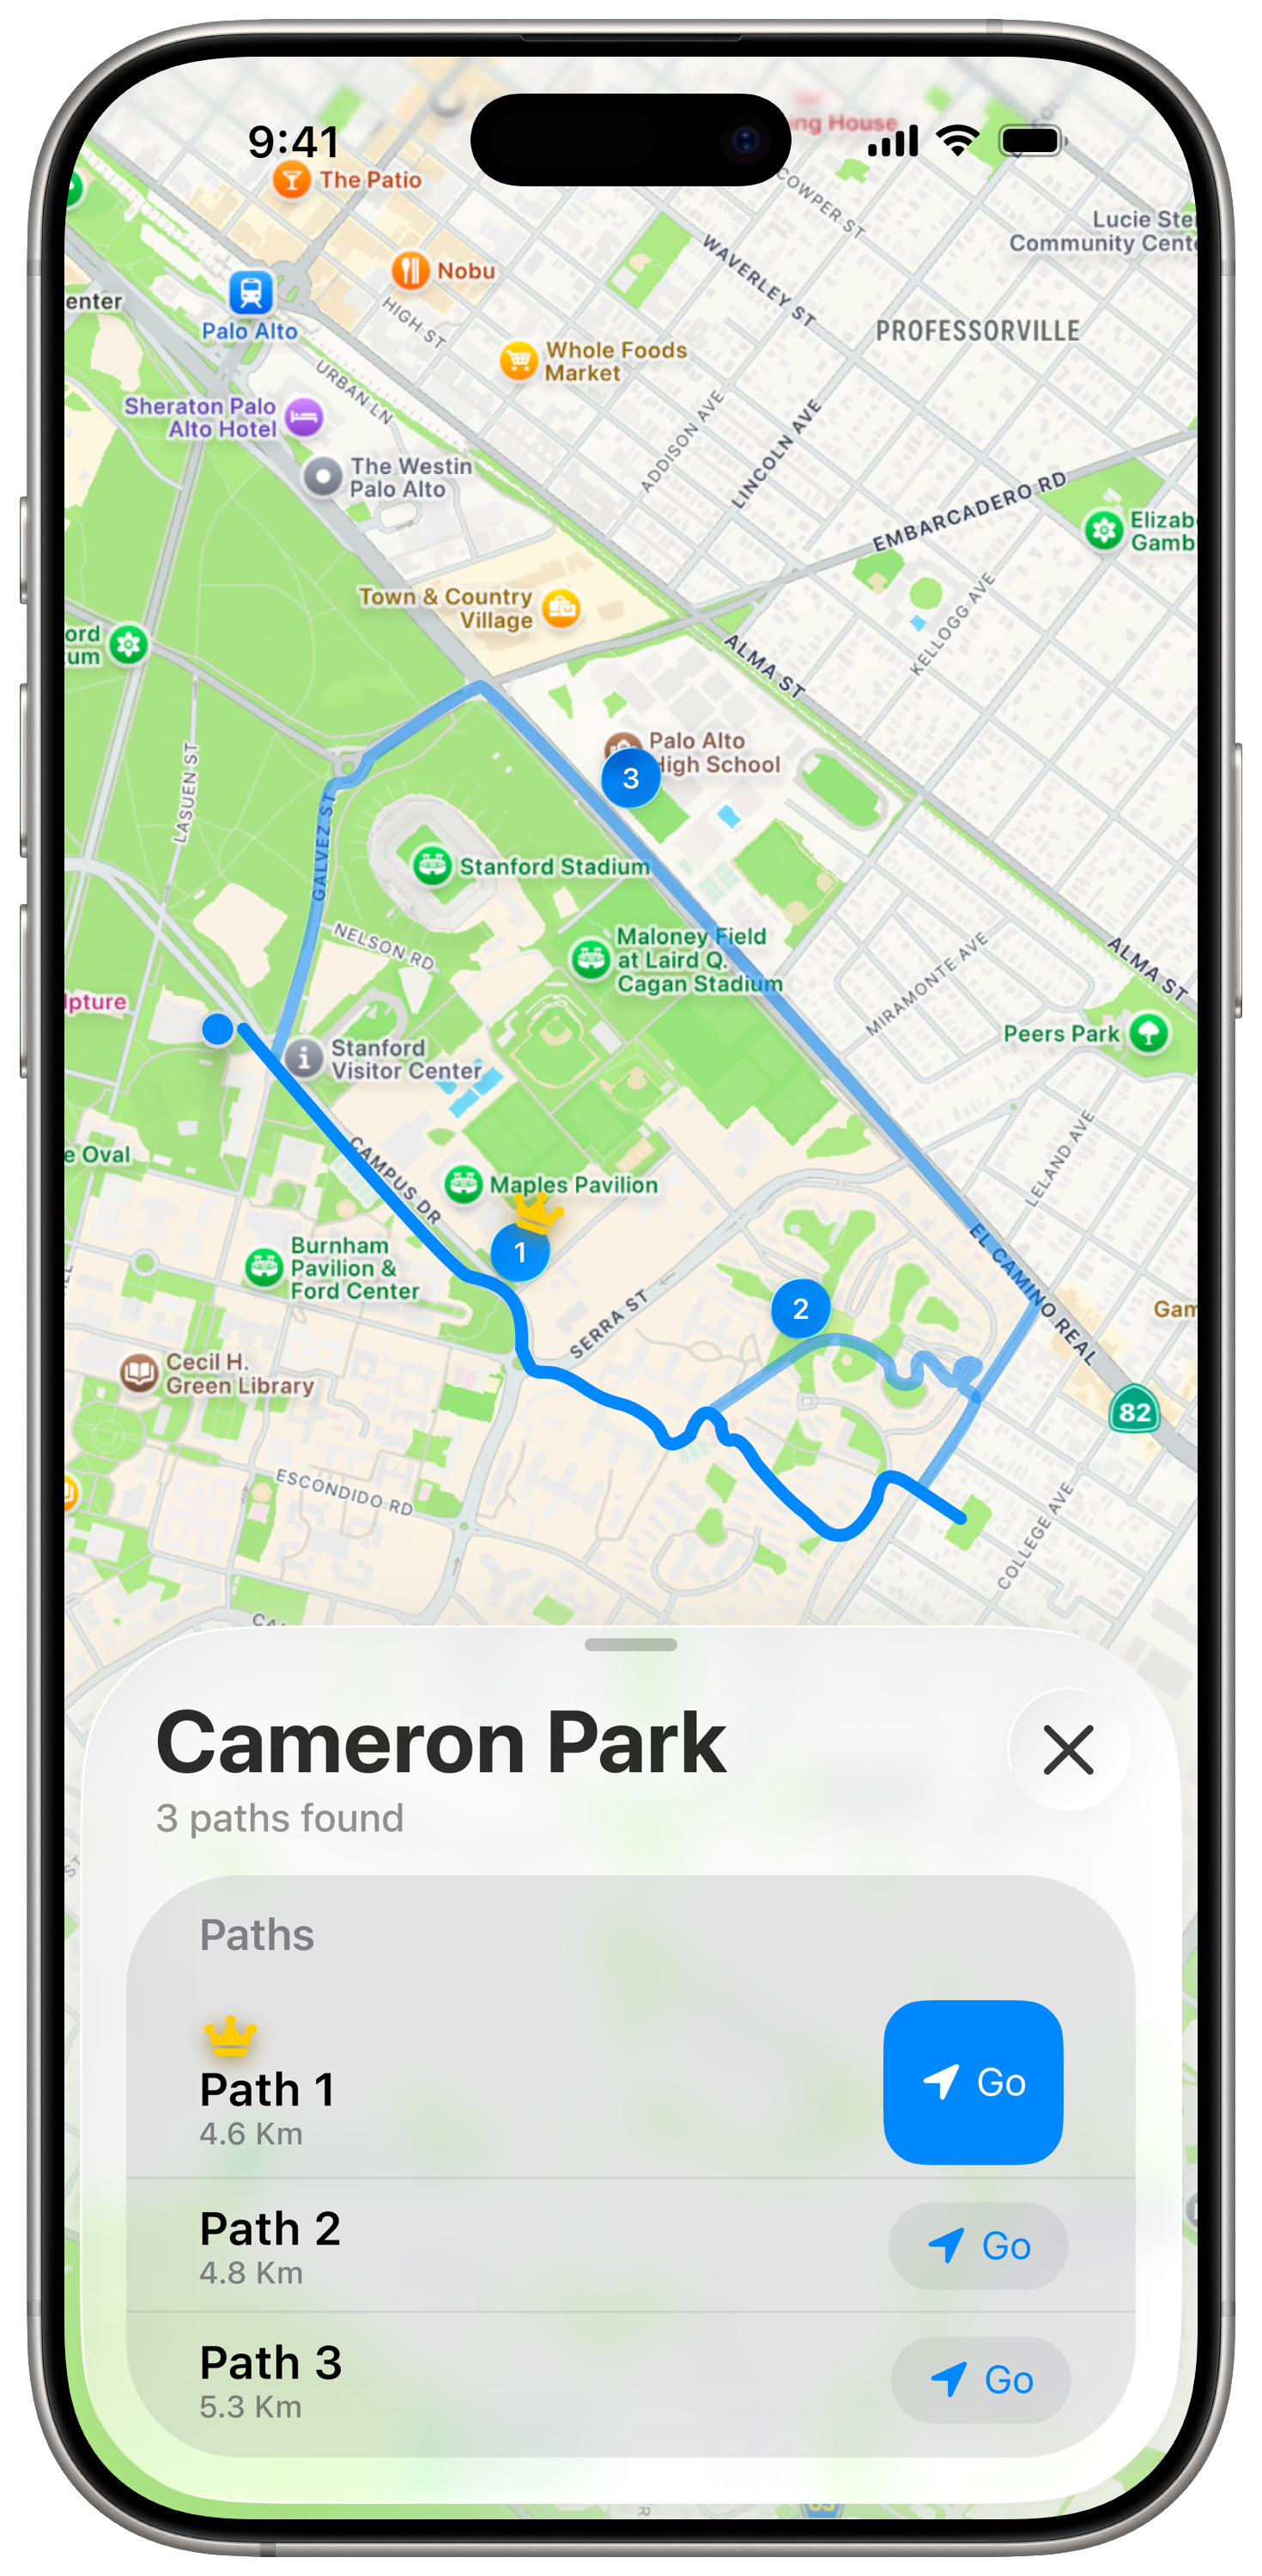
\includegraphics[width=\textwidth]{Mockups/ShowPaths_Map.PNG}
                \caption{Show Paths}
                \label{fig:show_paths_map}
            \end{subfigure}
        \end{figure}

    \subsection{Trip recording}
        From the Path selection screen, Users can choose any of the proposed Paths and start a Trip that guides them to the selected destination by following that Path.

        BBP is designed to be more than a fitness tracker: it provides turn-by-turn navigation to safely guide Users along their route. Since the application is intended to be used while the User is effectively driving a vehicle (i.e., riding a bike), it must comply with relevant safety regulations and standards, in particular ISO 9241, which defines principles for safe interaction with devices during driving-related activities.

        For this reason, BBP adopts a minimal and distraction-free navigation interface. The view focuses on the map and the currently followed Path, clearly highlighting the User’s position and the streets to be ridden next, rather than displaying the entire route at once.

        The map perspective automatically adapts to the current context, switching between a top-down view and a street-level view depending on which representation is most effective at that moment, helping users better understand their surroundings without requiring manual interaction.

        The next navigation instruction is prominently displayed in a top banner, combining textual and graphical cues. Less time-critical information, such as fitness-related data, is presented in a bottom sheet, which exposes only essential elements in its compact state and reveals additional details when expanded.

        To further discourage unsafe interaction while riding, no additional in-app actions are available in this view. The only available control is a prominent Stop button, which ends both the Trip recording and the turn-by-turn navigation.

        \begin{figure}[H]
            \centering
            \begin{subfigure}[b]{0.3\textwidth}
                \centering
                \includegraphics[width=\textwidth]{Mockups/Trip_Navigation.PNG}
                \caption{Top-down view}
                \label{fig:trip_recording1}
            \end{subfigure}
            \begin{subfigure}[b]{0.3\textwidth}
                \centering
                \includegraphics[width=\textwidth]{Mockups/Trip_Navigation2.PNG}
                \caption{Street-level view}
                \label{fig:trip_recording2}
            \end{subfigure}
        \end{figure}

    \subsection{Add Path - Manual}
        When Users intend to add a new Path to BBP, they are presented with two available modes: Manual and Automated.

        In Manual mode, Users are required to enter the Path data themselves. BBP provides a dedicated screen where users can either select a Path directly from the map, which can be expanded to full screen for improved usability, or search for a street by name to locate it that way.

        \begin{figure}[H]
            \centering
            \begin{subfigure}[b]{0.3\textwidth}
                \centering
                \includegraphics[width=\textwidth]{Mockups/AddPath_Manual_Screen.PNG}
                \caption{Add Path screen}
                \label{fig:add_path_manual_screen}
            \end{subfigure}
            \begin{subfigure}[b]{0.3\textwidth}
                \centering
                \includegraphics[width=\textwidth]{Mockups/SearchStreet.PNG}
                \caption{Search Street by name}
                \label{fig:search_street_view}
            \end{subfigure}
            \begin{subfigure}[b]{0.3\textwidth}
                \centering
                \includegraphics[width=\textwidth]{Mockups/AddPath_Manual_Info.PNG}
                \caption{Safety Info}
                \label{fig:add_path_info}
            \end{subfigure}
        \end{figure}

        Once a street is selected and deemed compatible (i.e., not already present in BBP’s database and not marked as incompatible), BBP creates a draft Path and presents it to the User for completion. At this stage, the User is asked to provide the remaining information, including additional details about the street (such as whether cars or pedestrians are allowed), the Path’s road quality, selected from a predefined set of options, and the presence of any Obstacles.

        \begin{figure}[H]
            \centering
            \begin{subfigure}[b]{0.3\textwidth}
                \centering
                \includegraphics[width=\textwidth]{Mockups/PathDraft.PNG}
                \caption{Path Draft}
                \label{fig:path_draft_screen}
            \end{subfigure}
            \begin{subfigure}[b]{0.3\textwidth}
                \centering
                \includegraphics[width=\textwidth]{Mockups/PathDraft-StatePicker.png}
                \caption{Set Path state}
                \label{fig:path_draft_state_picker}
            \end{subfigure}
        \end{figure}

        Obstacle input is handled on a dedicated screen featuring a full-screen map. Users can add Obstacle markers via a button and drag them to the correct location along the highlighted Path. Tapping on an Obstacle marker allows the User to change its type, selected from a predefined set of options.

        \begin{figure}[H]
            \centering
            \begin{subfigure}[b]{0.3\textwidth}
                \centering
                \includegraphics[width=\textwidth]{Mockups/AddObstacle_Map.PNG}
                \caption{Add Obstacle}
                \label{fig:add_obstacle_map}
            \end{subfigure}
            \begin{subfigure}[b]{0.3\textwidth}
                \centering
                \includegraphics[width=\textwidth]{Mockups/AddPathManual_ObstacleType.PNG}
                \caption{Set Obstacle type}
                \label{fig:obstacle_type_picker}
            \end{subfigure}
        \end{figure}

        Once all information is entered, the user is returned to the Draft screen. Pressing the save button in the toolbar prompts the user to choose between two options: Save as Draft, which keeps the Path private, or Save and Publish, which submits the Path for review and potential inclusion in the public database.

        \begin{figure}[H]
            \centering
            \begin{subfigure}[b]{0.3\textwidth}
                \centering
                \includegraphics[width=\textwidth]{Mockups/AddPath_Manual_Confirm.PNG}
                \caption{Save as Draft or Save and Publish}
                \label{fig:publish_path_popup}
            \end{subfigure}
        \end{figure}

    \newpage
    \subsection{Add Path - Automated}
        If the user chooses Automated Mode, BBP begins a Trip recording session and presents the same screen designed for use while riding. 

        The key difference is that no navigation instructions are provided, since the destination is not predetermined. The map remains visible, however, to help the user maintain orientation during the recording.

        \begin{figure}[H]
            \centering
            \begin{subfigure}[b]{0.3\textwidth}
                \centering
                \includegraphics[width=\textwidth]{Mockups/Path_Automatic.png}
                \caption{Record a Trip to save the Path}
                \label{fig:add_path_automated_screen}
            \end{subfigure}
        \end{figure}

\newpage

\section{Requirements Traceability}

\begin{tabular}{|l|p{12cm}|}
\hline
\textbf{Requirements} & 
\textbf{R1}: The system shall provide statistics about each trip, including weather information (if available), distance, average speed, and related metrics.\newline
\textbf{R6}: The system shall record data from device sensors during a tracking session.\newline
\textbf{R7}: The system shall reconstruct a path based on the GPS data collected during the tracking session.\newline
\textbf{R8}: The system shall detect sudden anomalies in sensor data and associate them with potential obstacles along the path.\newline
\textbf{R9}: The system shall present the recorded data to the user at the end of the trip, requesting confirmation or correction. \\
\hline
\textbf{Components} & Mobile app \newline
API \newline
Record Trip Service \newline
User Management Service \newline
Navigation Service \\
\hline
\end{tabular}

\begin{tabular}{|l|p{12cm}|}
\hline
\textbf{Requirements} & 
\textbf{R2}: Users shall be able to insert and publish information about bike paths, including their status and the presence of obstacles.\newline
\textbf{R3}: Users shall be able to manually insert paths by specifying street names.\newline
\textbf{R4}: The system shall translate street names into GPS coordinates and store the path information.\newline
\textbf{R5}: Users shall be able to start a tracking activity on their mobile device prior to a bike ride, instructing the system to record the path of their trip.\newline
\textbf{R6}: The system shall record data from device sensors during a tracking session.\newline
\textbf{R7}: The system shall reconstruct a path based on the GPS data collected during the tracking session.\newline
\textbf{R8}: The system shall detect sudden anomalies in sensor data and associate them with potential obstacles along the path.\newline
\textbf{R9}: The system shall present the recorded data to the user at the end of the trip, requesting confirmation or correction.\newline
\textbf{R15}: During an automated tracking session, BBP shall analyze speed and sensor data to detect cycling activity, reconstruct the path, and identify potential obstacles. The session must be explicitly started by the user; no background automatic tracking is performed. Detected obstacles require user confirmation before publication. \\
\hline
\textbf{Components} & 
Mobile App\newline
API\newline
User Management Service\newline
Add Path Service\newline
Navigation Service\newline
Record Trip Service\newline
Search Street Service \\
\hline
\end{tabular}

\begin{tabular}{|l|p{12cm}|}
\hline
\textbf{Requirements} & 
\textbf{R10}: The system shall allow users to publish the path data after it has been recorded and confirmed. \\
\hline
\textbf{Components} & 
Mobile App\newline
API\newline
User Management Service\newline
Path Review Management Service \\
\hline
\end{tabular}

\begin{tabular}{|l|p{12cm}|}
\hline
\textbf{Requirements} & 
\textbf{R11}: Users shall be able to query available paths given an origin and destination.\newline
\textbf{R12}: The system shall visualize all available paths on a map, given two locations (origin and destination).\newline
\textbf{R13}: The system shall compute a score to evaluate the effectiveness of each path in reaching the destination.\newline
\textbf{R14}: The system shall rank multiple plausible paths based on their computed score. \\
\hline
\textbf{Components} & 
Mobile App\newline
API\newline
User Management Service\newline
Search Destination Service\newline
Search Path Service \\
\hline
\end{tabular}

\newpage

\section{Implementation, Integration \& Testing}

    \subsection{Overview}
        This chapter explains how the described platform will be implemented and tested. The primary goal of testing is to identify and resolve most of the bugs in the code developed by the team. A detailed description of the integration process of the system's components will be provided in section 5.3. In contrast, section 5.2 will focus on the key implementation strategies employed in the project.

    \subsection{Implementation Plan}
        \subsubsection{Features identification}
            Below is a brief description of the main system features, expressed in terms of the services deployed to support them.

         \begin{description}[leftmargin=0pt, style=nextline] 
            \item[\textbf{[F1] User Registration and Login}]
            This feature is supported by the Authentication Service, which is responsible for user account creation and authentication. The service handles identity validation both internally and through external Single Sign-On (SSO) providers.
            
            \item[\textbf{[F2] User Management}]
            This feature is supported by the User Management Service, which manages all user-related data stored in the system. It provides access to profile information, path drafts, trip history, favourite and recent locations, and other user-specific data.
            
            \item[\textbf{[F3] Path Management}]
            This feature is supported by a set of services responsible for managing Paths and their lifecycle. These include components dedicated to querying Streets and Destinations, services for creating and managing Path drafts, and a dedicated service for handling the Path Review queue and approval process.
            
            \item[\textbf{[F4] Path Search}]
            This feature is supported by the Path Search Service, which implements the path-finding logic. The service generates routes between pairs of coordinates or locations by leveraging the database of previously created and validated Paths.
            
            \item[\textbf{[F5] Trip Management}]
            This feature is supported by two services designed to operate in conjunction. One service manages turn-by-turn navigation during an active Trip, while the other handles post-trip processing, including the persistence of Trip data and the update of Path-related information when applicable.
            
            \end{description}

        \subsection{Component Integration and Testing}
            In this section, we present the Deployment Diagram, which illustrates the physical architecture of the system and the allocation of software components to the underlying execution environments. The diagram reflects the incremental introduction of system features, where each addition may require the deployment of new components or the extension of previously deployed ones.

            The DBMS and the underlying database are not explicitly represented in the diagram, as they are assumed to be already deployed, configured, and operational at the time each feature is introduced. Similarly, external components and services are omitted, since they are outside the system boundary and are assumed to operate independently of the system under analysis.

            \begin{figure}[H]
                \textbf{[F1] User Registration and Login}\par\vspace{1em}
                \justifying
                The first feature to be deployed is the internal Authentication Service, which is responsible for handling user registration and authentication. The service supports both internal accounts and external accounts through Single Sign-On (SSO) providers.\\

                Alongside the Authentication Service, the Push Notification Service is also deployed at this stage. Its inclusion facilitates the testing and validation of the Authentication Service by enabling the delivery of authentication-related notifications.

                \centering
                \includegraphics[width=0.3\textwidth]{Testing/Testing_1.png}
            \end{figure}

            \begin{figure}[H]
                \textbf{[F2] User Management}\par\vspace{1em}
                \justifying
                Following the deployment of the Authentication Service, the User Management Service is introduced. This component is responsible for managing user-related data and provides access to profile information, trip history, favourite locations, and other user-specific data stored in the database.

                \centering
                \includegraphics[width=0.6\textwidth]{Testing/Testing_2.png}
            \end{figure}

            \begin{figure}[H]
                \textbf{[F3] Path Management}\par\vspace{1em}
                \justifying
                Next, the business logic related to Paths is deployed. This step includes components dedicated to specific queries, such as Streets and Destinations, which are used in some Path-related application flows.

                In addition, two services are introduced to handle Path Creation and the Path Review Process, respectively.

                \centering
                \includegraphics[width=\textwidth]{Testing/Testing_3.png}
            \end{figure}

            \begin{figure}[H]
                \textbf{[F4] Search Paths}\par\vspace{1em}
                \justifying
                Once the Path-related components are in place, the Path Search Service is deployed. This service is responsible for searching and generating routes between two location points by leveraging the Path data created and managed by the previously deployed services.

                \centering
                \includegraphics[width=\textwidth]{Testing/Testing_4.png}
            \end{figure}

            \begin{figure}[H]
                \textbf{[F5] Trip Management}\par\vspace{1em}
                \justifying
                Once the Path functionality is complete, the focus shifts to Trips. At this stage, two services are deployed in parallel: one dedicated to managing turn-by-turn navigation during an active trip, and another responsible for handling trip data upon completion. The latter service primarily stores trip-related information in the database and updates Path-related data accordingly.


                \centering
                \includegraphics[width=\textwidth]{Testing/Testing_5.png}
            \end{figure}

            \begin{figure}[H]
                \textbf{Complete integration}\par\vspace{1em}
                \justifying
                Finally, the API Gateway is deployed and configured to expose the system’s services through a unified entry point. This enables end-to-end testing of the complete system and its integration with the client applications. Until this stage, clients have been developed in parallel using mock APIs; once the API Gateway is in place, they can be connected to the actual backend services for full integration testing.


                \centering
                \includegraphics[width=\textwidth]{Testing/Testing_6.png}
            \end{figure}

        \subsection{System Testing}
            The system is developed following incremental integration strategies, combining bottom-up and thread-based approaches.

            \begin{itemize}
                \item In the \textbf{bottom-up strategy}, individual services are implemented and tested first in isolation. Each service is verified using scaffolders and drivers that simulate API calls from other modules. Once a service is confirmed to function correctly, it is integrated with previously deployed services, allowing higher-level features to be tested progressively.
                \item The \textbf{thread strategy} focuses on integrating services along functional flows, combining components required to execute complete use cases. This ensures that interactions between multiple services are validated as soon as they become operational, even before the full system is completed.
            \end{itemize}

            During development, this combination allows for early detection of issues in both single services and their interactions. Services such as Path Search and Trip Management, which handle complex logic or large amounts of data, require extensive testing under realistic conditions to ensure stability and correctness.

            Once all services are implemented, the system undergoes a structured testing process:
            \begin{itemize}
                \item \textbf{Functional Testing:}\\
                Ensures that the deployed services satisfy all functional and non-functional requirements outlined in the design documents.
                \item \textbf{Performance Testing:}\\
                Evaluates system efficiency, identifying potential bottlenecks in inter-service communication, database access, or algorithm execution.
                \item \textbf{Usability Testing:}\\
                Assesses client-side accessibility, ease of use, and user interaction, critical for a system intended for a broad user base.
                \item \textbf{Load Testing:}\\
                Measures system behavior under expected traffic volumes and concurrent users, verifying that services scale appropriately without degradation.
                \item \textbf{Stress Testing:}\\
                Tests the system beyond normal operational limits to identify weak points and ensure resilience under extreme conditions.
            \end{itemize}

            By combining bottom-up and thread strategies, the system guarantees that every service is tested both independently and in concert with other components, supporting a robust, reliable, and maintainable deployment architecture.

        \subsection{Additional Specifications on Testing}
            Throughout the development of the system, user acceptance testing (UAT) will be performed to ensure that the application satisfies the needs and expectations of stakeholders and end-users. The UAT process will include distinct alpha and beta testing phases. During alpha testing, the system is evaluated internally by the development team and a small group of selected stakeholders, allowing critical issues to be identified and resolved at an early stage. During beta testing, a broader pool of users interacts with the system in real-world conditions, providing feedback on functionality, usability, and overall performance.

            Given the sensitivity of data and interactions with external services, security testing is treated as a priority. Early identification and remediation of vulnerabilities ensures the system is robust and protected against potential threats.

            While client applications are still under development, testing will be performed using mock APIs and simulated interfaces. This allows verification of service functionality, inter-service communication, and data flows without requiring a fully implemented client. Once the API Gateway is deployed, the actual client applications can be connected to the backend, enabling comprehensive end-to-end testing of the complete system.

            For future feature releases, a phased rollout strategy is recommended. New functionality is initially made available to a limited subset of users before being expanded to the entire user base. Prior to beginning the rollout, the feature can be integrated into the client’s UI but hidden behind a server-controlled feature flag. This ensures that the client fully supports the new interface and interactions while the feature is tested in a controlled environment. This strategy allows developers to monitor performance, detect potential issues early, and safely address them before exposing the feature to all users.

            All testing activities follow industry best practices and are fully documented, ensuring traceability of issues, resolutions, and verification results.

    \newpage

    \section{Effort Spent}
    \begin{table}[H]
        \centering
        \begin{tabular}{|c|c|c|c|c|c|}
        \hline
        \textbf{} & \textbf{Ch. 1} & \textbf{Ch. 2} & \textbf{Ch. 3} & \textbf{Ch. 4} & \textbf{Ch. 5} \\
        \hline
        Rodigari M. & 3 & 10 & 8 & 2 & 5 \\
        \hline
        Summa C. & 1 & 12 & 10 & 4 & 5 \\
        \hline
        
        \end{tabular}
        \label{tab:chapters}
    \end{table}

    \section{References}
        \begin{itemize}
            \item Software Engineering II course slides and assignment specification.
            \item Overleaf, used as the collaborative LaTeX authoring environment.
            \item Google Docs, used for early collaborative drafting.
            \item Figma, used for the creation of UI mockups.
            \item draw.io, used for all architecture diagrams.
            \item sequencediagrams.org, used for modeling sequence diagrams.
        \end{itemize}
        
\end{document}
